% String comparison for \fref
\makeatletter
\long\def\isequal#1#2{\pdf@strcmp{#1}{#2}}
\makeatother

% An reference index from an unspecified source
% usage: \iref{environment}{value}
% for example: \iref{equation}{75}
\newcommand{\iref}[2]{%
  \switch%
  \case{\isequal{#1}{equation}}%
    ({#2})%
  \otherwise%
    {#2}%
  \endswitch%
}

% A formatted reference from an unspecified source
% usage: \fref{environment}{value}
% for example: \fref{figure}{75}
\newcommand{\fref}[2]{%
  \switch%
  \case{\isequal{#1}{equation}}%
    Eq.~\iref{#1}{#2}%
  \case{\isequal{#1}{figure}}%
    Fig.~\iref{#1}{#2}%
  \case{\isequal{#1}{section}}%
    Section~\iref{#1}{#2}%
  \otherwise%
    \PackageError{fref}{
      \MessageBreak
      environment value >#2< unknown \MessageBreak
    }{possible values are: equation. \MessageBreak}%
  \endswitch%
}

% References to external figures, equations, etc.
% usage: \xref{key}{environment}{value}
% for example: \xref{roman12}{figure}{75}
\newcommand{\xref}[3]{\citet{#1} \fref{#2}{#3}}

% Fourier Transform to angular momentum space
\newcommand{\Four}[1]{\ensuremath{{\mathcal F}\left\{ {#1} \right\}}}
% Fourier Transform to frequency space
\newcommand{\Fourf}[1]{\ensuremath{{\mathcal F}_f\left\{ {#1} \right\}}}

% use e^{...} instead of exp ...
\renewcommand{\exp}[1]{\ensuremath{e^{#1}}}

% Symbol denoting the Langevin function
\newcommand{\Langevin}{\ensuremath{\mathcal{L}}}
% Symbol denoting big-O order of #1
\newcommand{\order}[1]{\ensuremath{\mathcal{O}\p({#1})}}

% Integral from #1 to #2 of #4 with respect to #3
\newcommand{\integral}[4]{\ensuremath{\int_{#1}^{#2} {#4} \dd{#3}}}
% Integral from -infty to +infty of #2 with respect to #1
\newcommand{\iInfInf}[2]{\integral{-\infty}{\infty}{#1}{#2}}
% Integral from 0 to +infty of #2 with respect to #1
% note that the second char in the name is a capital o, not a 0
% because ?Latex doesn't allow digits in command names
\newcommand{\iOInf}[2]{\integral{0}{\infty}{#1}{#2}}
% #3 evaluated at #2 and #1
\newcommand{\evaluated}[3]{\ensuremath{\left.{#3}\right|_{#1}^{#2}}}
% #2 evaluated at #1
\newcommand{\eval}[2]{\ensuremath{\left.{#2}\right|_{#1}}}
% evaluated at infty and -infty
\newcommand{\eInfInf}[1]{\evaluated{-\infty}{\infty}{#1}}
% evaluated at infty and 0
\newcommand{\eOInf}[1]{\evaluated{0}{\infty}{#1}}

% we do a lot of lim t_T -> infty, so macro that out
% lim as #1 -> infty
\newcommand{\limInf}[1]{\ensuremath{\lim_{{#1}\rightarrow \infty}}}
\newcommand{\limT}{\limInf{t_T}}
\newcommand{\normLimT}{\limT \frac{1}{t_T}\ } % '\ ' for a normal space
% lim as t_T -> infty of integral from -t_T/2 to t_T/2 of #1 with respect to t
\newcommand{\iLimT}[1]{\normLimT \integral{-t_T/2}{t_T/2}{t}{#1}}

\newcommand{\magSq}[1]{\ensuremath{\left|{#1}\right|^2}}
\newcommand{\PSD}{\ensuremath{\operatorname{PSD}}}

% complex conjugate
\newcommand{\conj}[1]{\ensuremath{\overline{#1}}}

% Symbol denoting the contour C
\newcommand{\C}{\ensuremath{\mathcal{C}}}
% Integral about contour C of #1 with respect to z
\newcommand{\iC}[1]{\integral{\C}{}{z}{#1}}
\newcommand{\Reals}{\ensuremath{\mathds{R}}}
\newcommand{\Imags}{\ensuremath{\mathds{I}}}
\newcommand{\Real}{\ensuremath{\operatorname{Re}}}
\newcommand{\Imag}{\ensuremath{\operatorname{Im}}}
\newcommand{\ResX}[3]{\operatorname{Res}\left({{#1}={#2}},{#3}\right)}
\newcommand{\Res}[2]{\ResX{z}{#1}{#2}}
\newcommand{\limX}[2]{\lim_{{#1} \rightarrow {#2}}}
\newcommand{\limZ}[1]{\limX{z}{#1}}
\newcommand{\limZp}{\limZ{z_p}}
\newcommand{\CPV}{\ensuremath{\mathds{P}}}

\newcommand{\supScript}[1]{\ensuremath{^{\text{#1}}}}
\newcommand{\st}{\supScript{st}}
\newcommand{\nd}{\supScript{nd}}
\newcommand{\rd}{\supScript{rd}}
\newcommand{\sth}{\supScript{th}} % th, TH already taken

\newcommand{\colA}[1]{\textcolor{red}{#1}}
\newcommand{\colB}[1]{\textcolor{blue}{#1}}
\definecolor{purple}{rgb}{0.8, 0, 0.8}
\newcommand{\colAB}[1]{\textcolor{purple}{#1}}
\newcommand{\colC}[1]{\textcolor{green}{#1}}

\newcommand{\cf}{\emph{cf.}} % "confer" or "bring together" / "compare"
\newcommand{\ie}{\emph{i.e.}} % "id est" or "in other words"
\newcommand{\insilico}{\emph{in silico}} % quasi latin for "on a computer"
\newcommand{\invitro}{\emph{in vitro}}   % latin for "in glass"
\newcommand{\invivo}{\emph{in vivo}}     % latin for "in living organisms"

\newcommand{\gui}[1]{\emph{#1}}  % highlighting for quotes from a GUI

\newcommand{\ensuretext}[1]{\ensuremath{\text{#1}}}
% Hyeon and Thirumalai equation number #1
\newcommand{\HTeq}[1]{\ensuretext{\emph{H\&T eq.\ {#1}}}}
\newcommand{\kT}{\ensuremath{k_B T}}
\newcommand{\bt}{\ensuremath{\beta}}
\newcommand{\fs}{\ensuremath{f^*}}
\newcommand{\dx}{\ensuremath{\Delta x(\fs)}}
\newcommand{\dxs}[1]{\ensuremath{\Delta x_{#1}(\fs)}} % for subscripting
\newcommand{\FO}{\ensuremath{\Delta F_0^\ddagger(\fs)}}
\newcommand{\vD}{\ensuremath{\nu_D(\fs)}}
\newcommand{\vDs}[1]{\ensuremath{\nu_{D{#1}}(\fs)}}
\newcommand{\kexp}{\ensuremath{\vD e^{-\bt \FO}}}
\newcommand{\kexps}[1]{\ensuremath{\vDs{#1} e^{-\bt_{#1} \FO_{#1}}}}
\newcommand{\kf}{\ensuremath{k(\fs)}}
\newcommand{\kfs}[1]{\ensuremath{k_{#1}(\fs)}}
%\newcommand{\avg}[1]{\ensuremath{\left\langle {#1} \right\rangle}}
\newcommand{\abs}[1]{\ensuremath{\lvert {#1} \rvert}}
\newcommand{\logp}[1]{\ensuremath{\log\!\!\left( {#1} \right)}}
% \! is a negative thin space to get the paren closer to the log
%\renewcommand{\r}{\ensuremath{r_f}}
%\newcommand{\rs}[1]{\ensuremath{r_{f{#1}}}}% to avoid double-subscripting
\newcommand{\ep}{\varepsilon}

\newcommand{\species}[1]{\emph{#1}} % \species{Homo sapiens}

% Chemicals
\newcommand{\Ca}{Ca\textsuperscript{2+}}
\newcommand{\CaCl}{CaCl\textsubscript{2}}
\newcommand{\Cu}{Cu\textsuperscript{2+}}
\newcommand{\Cl}{Cl\textsuperscript{-}}
\newcommand{\HCl}{HCl}
\newcommand{\KCl}{KCl}
\newcommand{\MgCl}{MgCl\textsubscript{2}}
\newcommand{\Na}{Na\textsuperscript{+}}
\newcommand{\NaCl}{NaCl}
\newcommand{\diNaHPO}{Na\textsubscript{2}HPO\textsubscript{4}}
\newcommand{\NadiHPO}{NaH\textsubscript{2}PO\textsubscript{4}}
\newcommand{\NaOH}{NaOH}

% Workaround for inline minted markup
%   http://code.google.com/p/minted/issues/detail?id=15
% usage: \imint{language}|value|
\NewDocumentCommand\imint{mv}{\texttt{#2}}

% Aliases for citations
\defcitealias{calibcant}{calibcant}
\defcitealias{comedi}{Comedi}
\defcitealias{cygwin}{Cygwin}
\defcitealias{cython}{Cython}
\defcitealias{epics}{EPICS}
\defcitealias{force-robot}{ForceRobot}
\defcitealias{gentoo}{Gentoo}
\defcitealias{git}{Git}
\defcitealias{h5config}{h5config}
\defcitealias{hdf5}{HDF5}
\defcitealias{interix}{Interix}
\defcitealias{kernighan88}{C}
\defcitealias{king10}{sawsim}
\defcitealias{labview}{LabVIEW}
\defcitealias{picoforce}{PicoForce}
\defcitealias{prefix}{Gentoo Prefix}
\defcitealias{punias}{PUNIAS}
\defcitealias{pyafm}{pyafm}
\defcitealias{pycomedi}{pycomedi}
\defcitealias{pymodbus}{pymodbus}
\defcitealias{pymol}{PyMol}
\defcitealias{pypid}{pypid}
\defcitealias{pypiezo}{pypiezo}
\defcitealias{python}{Python}
\defcitealias{sandal09}{Hooke}
\defcitealias{stepper}{stepper}
\defcitealias{beazley96}{SWIG}
\defcitealias{unfold-protein}{unfold-protein}
\defcitealias{wavemetrics-igor}{IGOR Pro}
\defcitealias{xcode}{Xcode}
\defcitealias{yaml}{YAML}

\newcommand{\Comedi}{\citetalias{comedi}}
\newcommand{\Hooke}{\citetalias{sandal09}}
\newcommand{\calibcant}{\citetalias{calibcant}}
\newcommand{\hFconfig}{\citetalias{h5config}}
\newcommand{\pyafm}{\citetalias{pyafm}}
\newcommand{\pypid}{\citetalias{pypid}}
\newcommand{\pypiezo}{\citetalias{pypiezo}}
\newcommand{\pycomedi}{\citetalias{pycomedi}}
\newcommand{\pysawsim}{\texttt{pysawsim}}
\newcommand{\sawsim}{\citetalias{king10}}
\newcommand{\stepper}{\citetalias{stepper}}
\newcommand{\unfoldprotein}{\citetalias{unfold-protein}}

% draw a line TikZ (useful for captions explaining figures)
% usage: \tikzline{style}
\DeclareRobustCommand{\tikzline}[1]{%
  \protect\tikz \draw[#1] (0,0) -- (14pt,6pt);}

\DeclareRobustCommand{\thermocouple}{%
  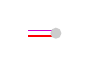
\begin{tikzpicture}
    \draw[red] (0,1pt) -- (10pt,1pt);
    \draw[purple] (0,3pt) -- (10pt,3pt);
    \fill[black!20] (10pt,2pt) circle (2pt);
  \end{tikzpicture}
}

% draw a thermometer in TikZ
% usage: \thermometerx{bulb-location}
\newcommand{\thermometerx}[1]{
  \draw[blue!20, line width=4pt, cap=round] #1 -- +(0, 12pt);
  \fill[blue!20] #1 circle (5pt);
  \draw[red, line width=2pt, cap=butt] #1 -- +(0, 8pt);
  \fill[red] #1 circle (4pt);
}

\DeclareRobustCommand{\thermometer}{%
  \raisebox{-2pt}{%
    \resizebox{!}{10pt}{%
      
\begin{tikzpicture}%
        \thermometerx{(0,2.5pt)};%
      \end{tikzpicture}%
    }%
  }%
}

% shared figure between pyafm and calibcant
% usage: \tikzstack{unfold-protein-color}{calibcant-color}
\newcommand{\tikzstack}[2]{%
  \begin{tikzpicture}[decoration={
      markings,%  switch on markings
      mark=%  add a mark for screw threading
        between positions 0 and 1 step 1pt
        with
        {
          \draw (0, 2pt) -- (1pt, -2pt);
        }
      },
      bend angle=5
      ]
    \tikzstyle{every node}=[text depth=0pt, rounded rectangle,
      draw=blue!50, very thick, minimum height=1.7em]
    % hardware nodes and coordinates
    \node[shape=rectangle,draw=none,inner sep=0]
      (image) at (0,0) {
      \asyinclude{figures/schematic/afm}};
    \node[shape=rectangle,draw=black, semithick]
      (daq) at ($(image.south west) + (-0.25, -1)$) {DAQ card};
    \node[shape=rectangle,draw=black, semithick]
      (motor) at ($(image.south) + (0, -1)$) {motor};
    \coordinate (thermocouple) at ($(image.west) + (1.4, -4pt)$);
    \thermometerx{(thermocouple)}
    \coordinate (photodiode) at ($(image.west) + (1, 26pt)$);
    \coordinate (piezo) at ($(image.south) + (-6pt, 0)$);
    \draw[black!20,dashed] ($(daq.south west) + (-10pt, 0)$) -- +(0, 4);
    % software nodes
    \node (pycomedi) at ($(daq) + (-6,0)$) {pycomedi};
    \node (pypiezo) at ($(pycomedi) + (0,1)$) {pypiezo};
    \node (pyafm) at ($(pypiezo) + (0,1)$) {pyafm};
    \node[#1] (unfold-protein) at ($(pyafm) + (0,1)$) {unfold-protein};
    \node (stepper) at ($(pycomedi) + (2,1)$) {stepper};
    \node (pypid) at ($(stepper) + (2,0)$) {pypid};
    \node (h5config) at ($(pycomedi) + (-3,0)$) {h5config};
    \node[#2] (calibcant) at ($(unfold-protein) + (-3,0)$) {calibcant};
    % software connections
    \draw (pypiezo) -- (pyafm);
    \draw (stepper) -- (pyafm);
    \draw (pypid) -- (pyafm);
    \draw[#1] (pyafm) -- (unfold-protein);
    \draw (h5config) -- (pypiezo);
    \draw (h5config) -- (pyafm);
    \ifthenelse{\equal{#1}{}}{%  draw unfold-protein in black (the default)
      \draw[#2] (pyafm) -- (calibcant);
      \draw[#1] (h5config) -- (unfold-protein);%  default path on top
      }{%
      \draw[#1] (h5config) -- (unfold-protein);
      \draw[#2] (pyafm) -- (calibcant);%  default path on top
      }
    \draw[#2] (h5config) -- (calibcant);
    % hardware connections
    \begin{pgfonlayer}{background}
      \draw[purple, ->] (thermocouple) -- (pypid);
    \end{pgfonlayer}
    % begin motor screw
    \draw[black!20, line width=4pt]
      (motor) -- (image.south);   % shaft with decoration threads
    \draw[black, decorate, ultra thin]
      (motor) -- (image.south);   % shaft with decoration threads
    % end motor screw
    \draw[red, <->] (pypiezo) -- (pycomedi);
    \draw[red, <->] (pycomedi) to [bend left] (daq);
    \draw[red, ->] (daq) -- (piezo);
    \begin{pgfonlayer}{background}
      \draw[red, ->, out=180, in=90] (photodiode) to (daq.north);
    \end{pgfonlayer}
    \draw[blue, ->] (stepper) -- (pycomedi);
    \draw[blue, ->] (pycomedi) to [bend right] (daq);
    \draw[blue, ->] (daq) -- (motor);
  \end{tikzpicture}
}
